%\documentclass[compress]{beamer}
\documentclass[8pt]{beamer}

%-----------------------------------------------------------
% PACKAGES
\usepackage{graphicx}   % for graphics

%\usepackage[latin1]{inputenc}
\mode<presentation>

%\usepackage[T1]{fontenc}  
\usetheme{Warsaw}
%\usetheme{Madrid}

\usepackage{graphicx}
%\usepackage[section]{placeins} % force � mettre l'image o� on veut
%\usepackage{float} %utiliser H pour forcer � mettre l'image o� on veut
%\usepackage{lscape} %utilisation du mode paysage
%\usepackage{pslatex}
\usepackage{url}
\usepackage{subfigure}
\usepackage{caption}
%\usepackage{subcaption}
%\usepackage[caption=false]{subfig}

\usepackage{graphicx}
\usepackage{tabls}
\usepackage{afterpage}

%\usepackage[]{media9}
%\usepackage{multimedia}

\usepackage{amsthm}
\usepackage{amssymb}
\usepackage{amsmath}
\usepackage{amsfonts}
\usepackage{amstext}
\usepackage{amsbsy}
\usepackage{mathbbol} 


\usepackage{epsfig}
%\usepackage{epsfig}
%\usepackage{cites}
\usepackage{epsf}
\usepackage{array}
\usepackage{color}

%-----------------------------------------------------------
% NEW  DEFINITIONS

%=================================================================================================

%============================================================

%style et couleur
%\usetheme{Frankfurt}
\date{\today}

%\addtobeamertemplate{footline}{\hfill\insertframenumber/\inserttotalframenumber\hspace{2em}\null}

\setbeamertemplate{footline}{
\leavevmode%
%\hbox{\hspace*{-0.06cm}
\begin{beamercolorbox}[wd=.5\paperwidth,ht=3.25ex,dp=1ex,center]{author in head/foot}%
	\usebeamerfont{author in head/foot}\insertshortauthor%~~(\insertshortinstitute)
\end{beamercolorbox}%
\begin{beamercolorbox}[wd=.25\paperwidth,ht=3.25ex,dp=1ex,center]{section in head/foot}%
	\usebeamerfont{section in head/foot} April 2016 % \insertshorttitle
\end{beamercolorbox}%
\begin{beamercolorbox}[wd=.25\paperwidth,ht=3.25ex,dp=1ex,left]{section in head/foot}%
	\usebeamerfont{section in head/foot}\insertshortdate{}\hspace*{2em}
	\insertframenumber{} / \inserttotalframenumber %\hspace*{2ex}
\end{beamercolorbox}}%
%\vskip0pt%
%}

\beamertemplatetransparentcovered


%\title{Entropy-based artificial viscosity stabilization for non-equilibrium Grey 
%Radiation-Hydrodynamics}
\title{RadHy convergence plots}

\author{JCR MOD}
\vspace{5mm}
\institute{{\large  Texas A\&M University, College Station, TX, USA}}

%%%%%%%%%%%%%%%%%%%%%%%%%%%%%%%%%%%%%%%%%%%%%%%%%%%%%%%%%%%%%%%%%%%%

\begin{document}

\begin{frame}
\titlepage
\end{frame}

%\begin{frame}
	%\frametitle{Outline}
	%\tableofcontents 
%\end{frame}


%%%%%%%%%%%%%%%%%%%%%%%%%%%%%%%%%%%%%%%%%%%%%%%%%%%%%%%%%%%%%%%%%%%%%%%%%%%%%%%%%
\begin{frame}
\frametitle{Mach 1.05}

% path to figures directory
\newcommand{\FiguresDirnew}{./March31/Mach-1.05}
\setcounter{subfigure}{0}% Reset subfigure counter
\small{First email, 3/31. Maybe not small enough time step. Legend is wrong (ref. slope is 2) CFL=???}

\begin{figure}[h]
   \centering
\subfigure[Density]{
      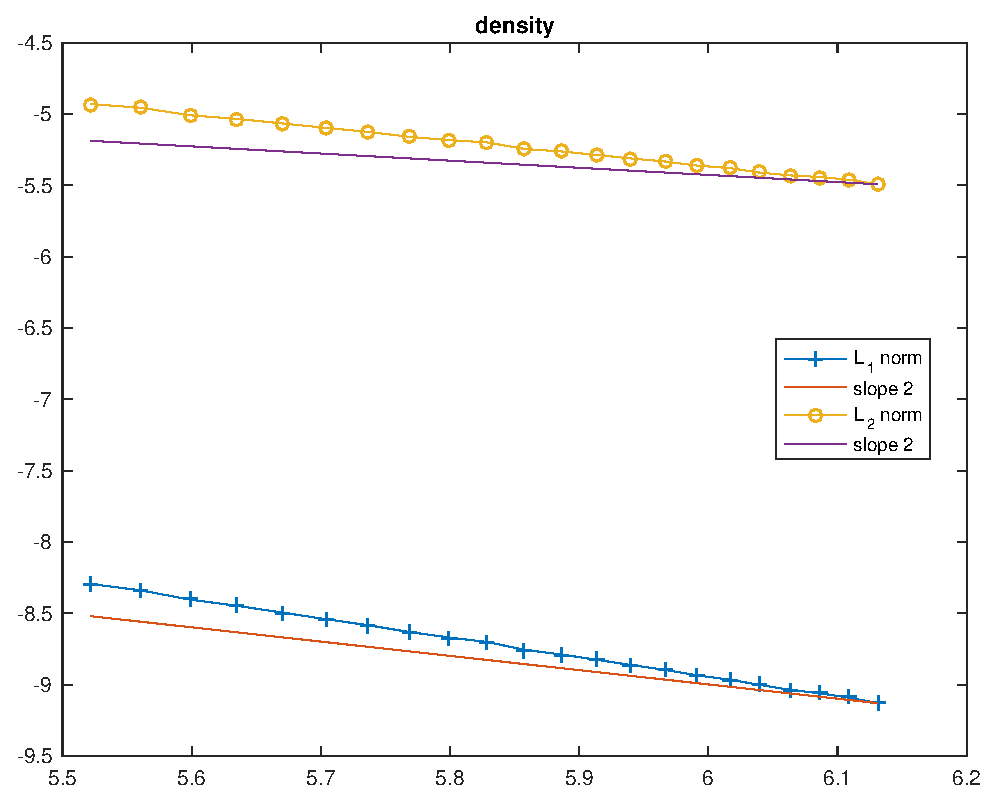
\includegraphics[width=0.4\textwidth]{\FiguresDirnew/density_pchip.eps}
}
\hspace{1cm}
\subfigure[Mach]{
      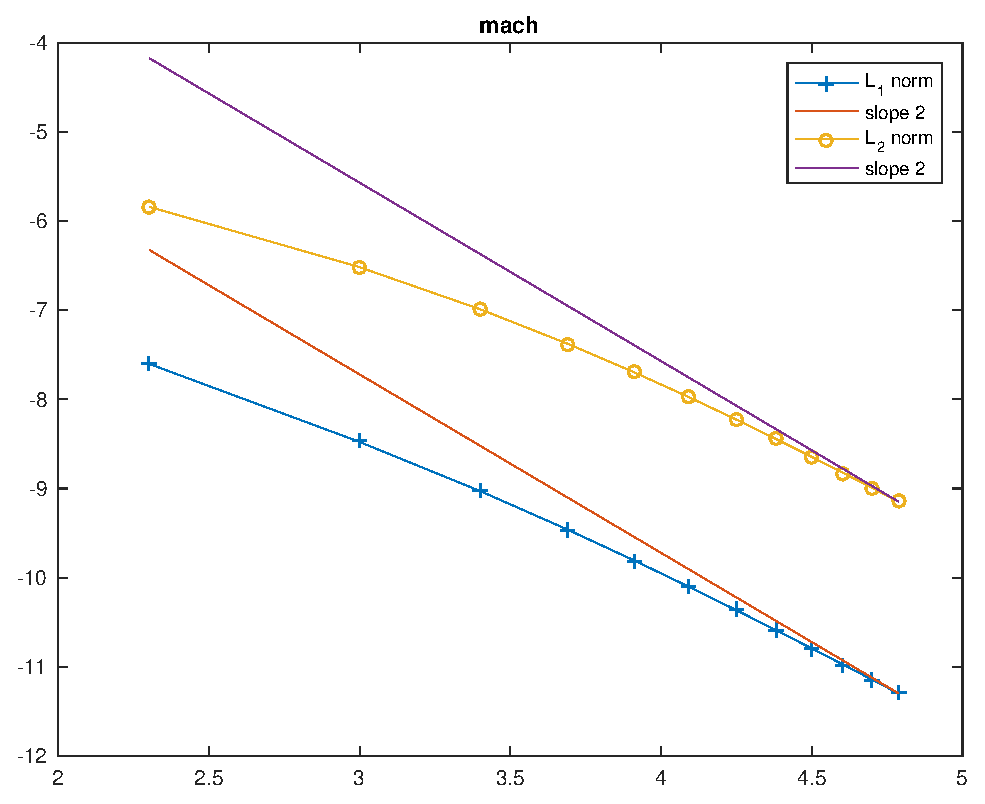
\includegraphics[width=0.4\textwidth]{\FiguresDirnew/mach_pchip.eps}
}
\subfigure[Mat. Temp.]{
      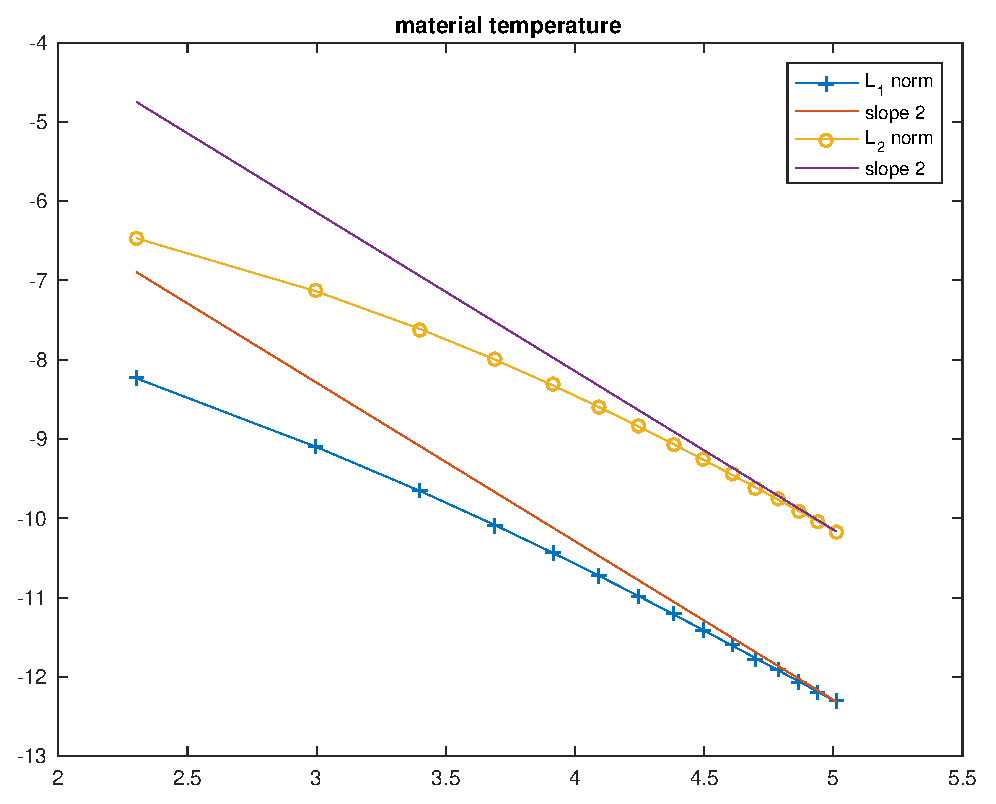
\includegraphics[width=0.4\textwidth]{\FiguresDirnew/material_temperature_pchip.eps}
}
\hspace{1cm}
\subfigure[Radiation Temp.]{
      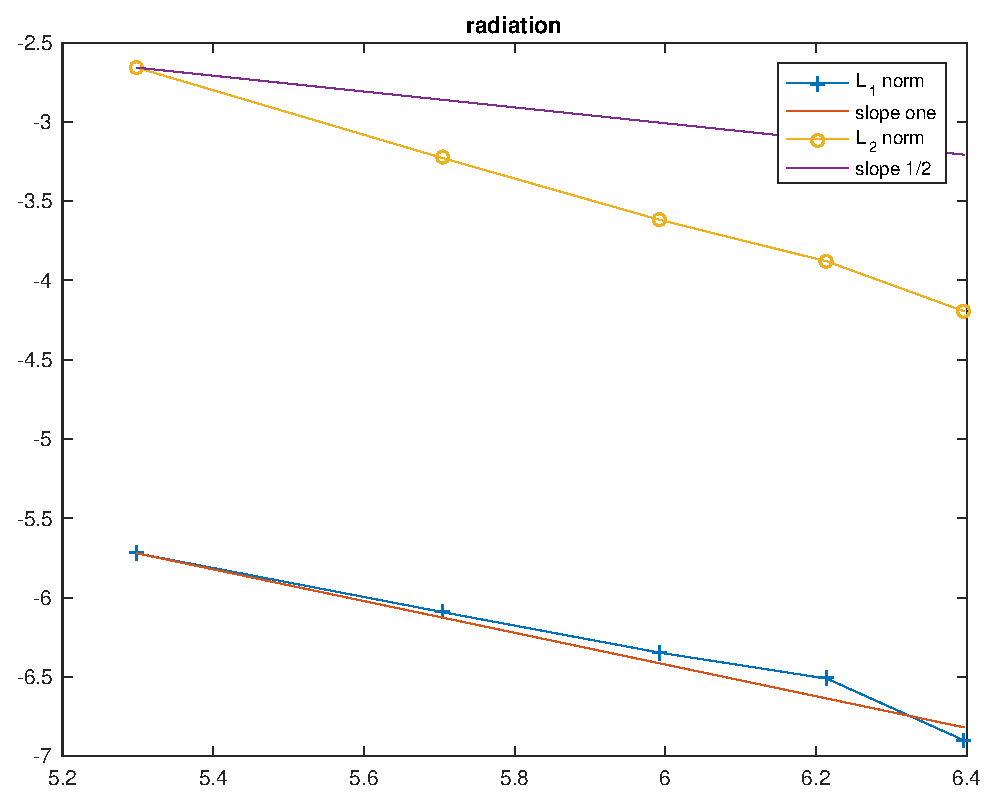
\includegraphics[width=0.4\textwidth]{\FiguresDirnew/radiation_pchip.eps}
}
\end{figure}

\end{frame}
%%%%%%%%%%%%%%%%%%%%%%%%%%%%%%%%%%%%%%%%%%%%%%%%%%%%%%%%%%%%%%%%%%%%%%%%%%%%%%%%%

%%%%%%%%%%%%%%%%%%%%%%%%%%%%%%%%%%%%%%%%%%%%%%%%%%%%%%%%%%%%%%%%%%%%%%%%%%%%%%%%%
\begin{frame}
\frametitle{Mach 1.05}

% path to figures directory
\newcommand{\FiguresDirnew}{./April4/Mach-1.05}
\setcounter{subfigure}{0}% Reset subfigure counter
\small{New results, April 4-5. Same setting as other Mach 1.05 but CFL=0.02 now}

\begin{figure}[h]
   \centering
\subfigure[Density]{
      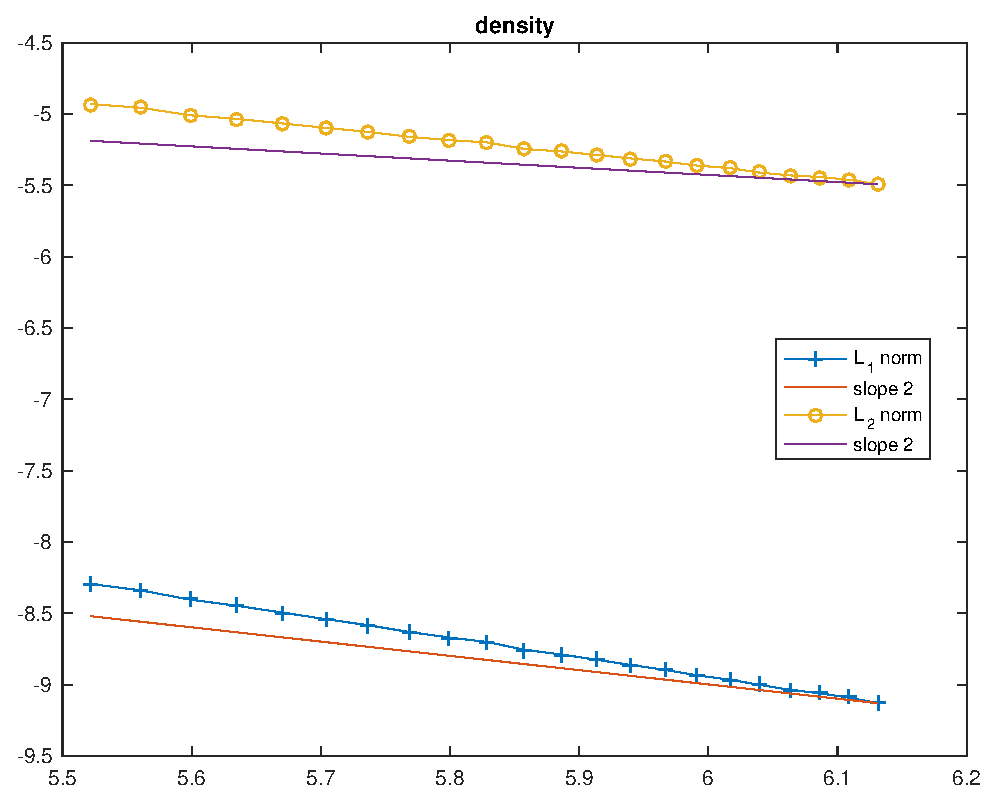
\includegraphics[width=0.4\textwidth]{\FiguresDirnew/density_pchip.eps}
}
\hspace{1cm}
\subfigure[Mach]{
      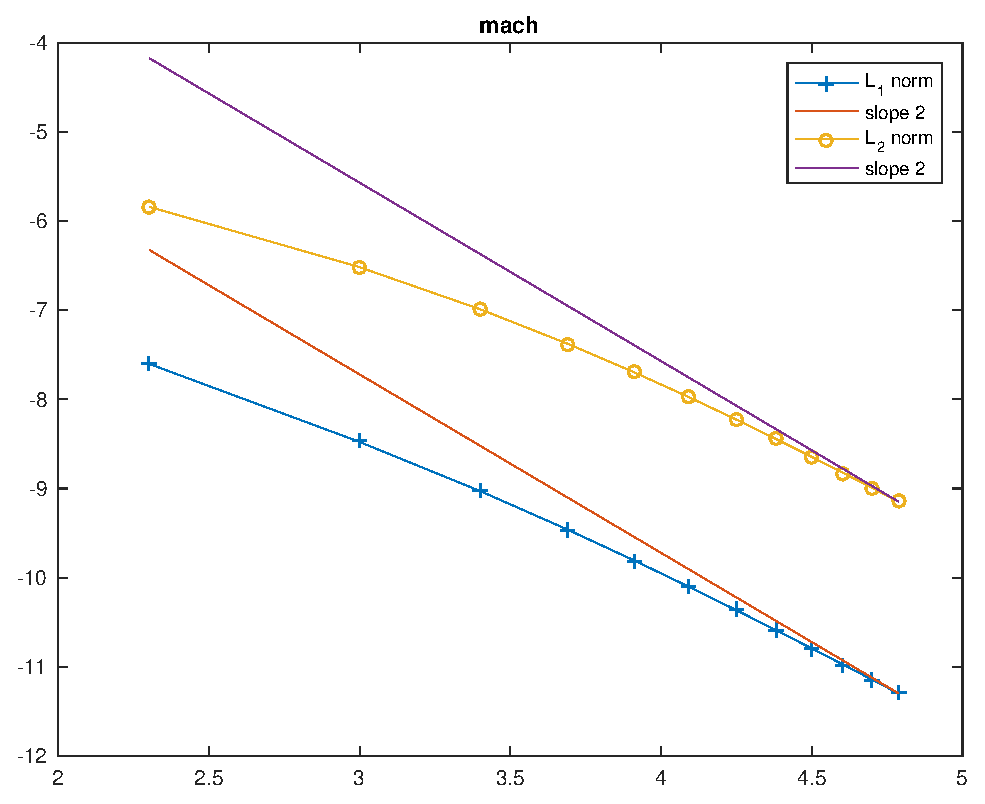
\includegraphics[width=0.4\textwidth]{\FiguresDirnew/mach_pchip.eps}
}
\subfigure[Mat. Temp.]{
      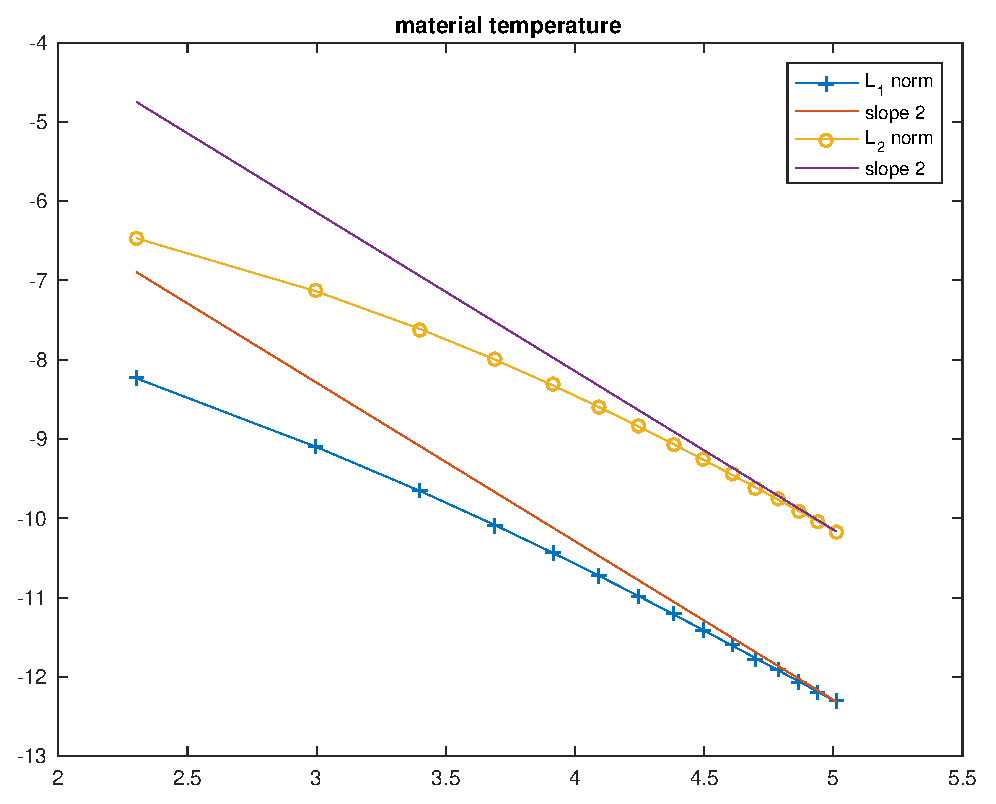
\includegraphics[width=0.4\textwidth]{\FiguresDirnew/material_temperature_pchip.eps}
}
\hspace{1cm}
\subfigure[Radiation Temp.]{
      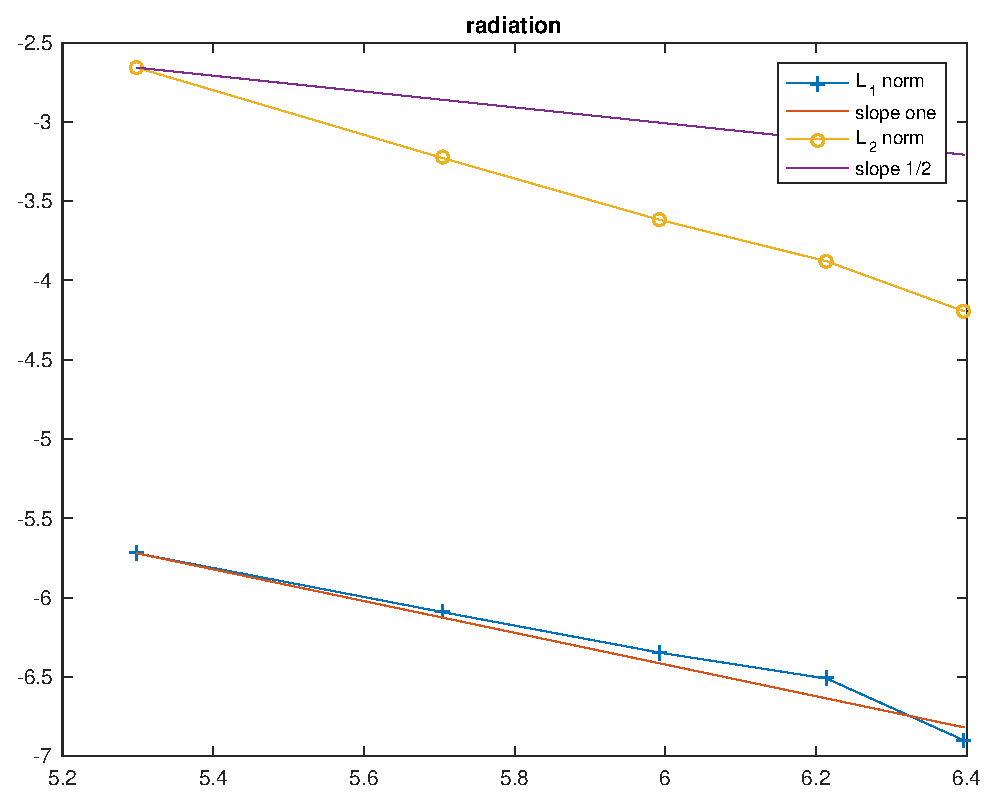
\includegraphics[width=0.4\textwidth]{\FiguresDirnew/radiation_pchip.eps}
}
\end{figure}

\end{frame}
%%%%%%%%%%%%%%%%%%%%%%%%%%%%%%%%%%%%%%%%%%%%%%%%%%%%%%%%%%%%%%%%%%%%%%%%%%%%%%%%%

%%%%%%%%%%%%%%%%%%%%%%%%%%%%%%%%%%%%%%%%%%%%%%%%%%%%%%%%%%%%%%%%%%%%%%%%%%%%%%%%%
\begin{frame}
\frametitle{Mach 3}

% path to figures directory
\newcommand{\FiguresDirnew}{./March31/Mach-3}
\setcounter{subfigure}{0}% Reset subfigure counter
\small{First email, March 31. Maybe not small enough time step. CFL=??? Opacities NOT dependent on temp??}

\begin{figure}[h]
   \centering
\subfigure[Density]{
      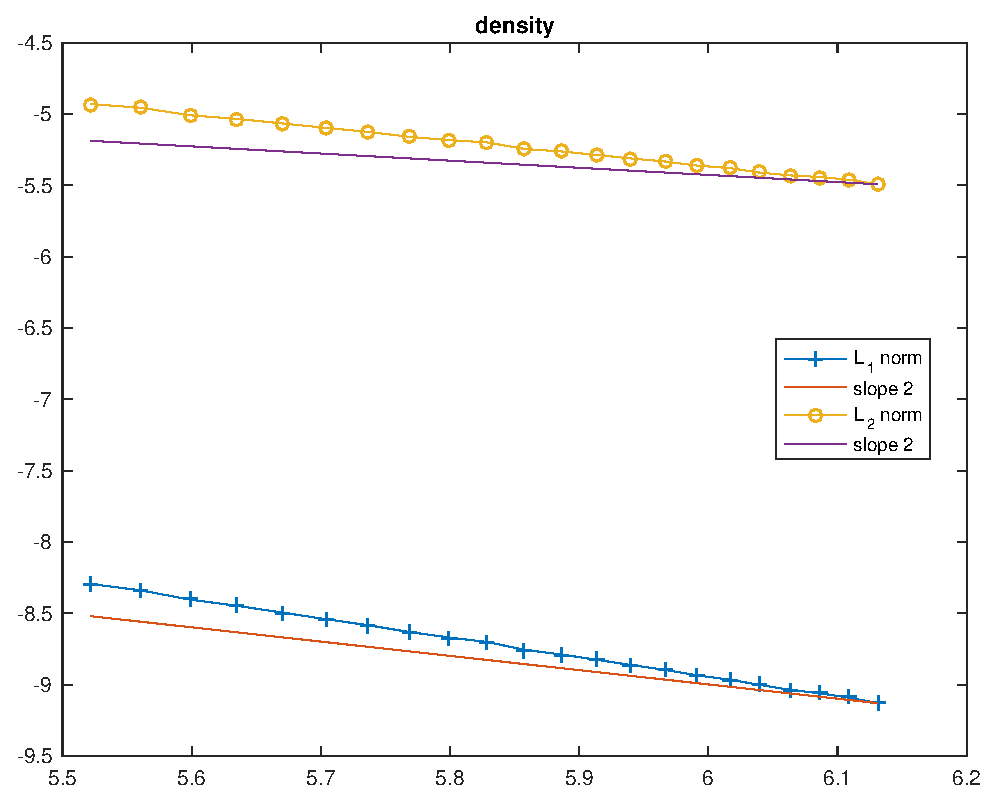
\includegraphics[width=0.4\textwidth]{\FiguresDirnew/density_pchip.eps}
}
\hspace{1cm}
\subfigure[Mach]{
      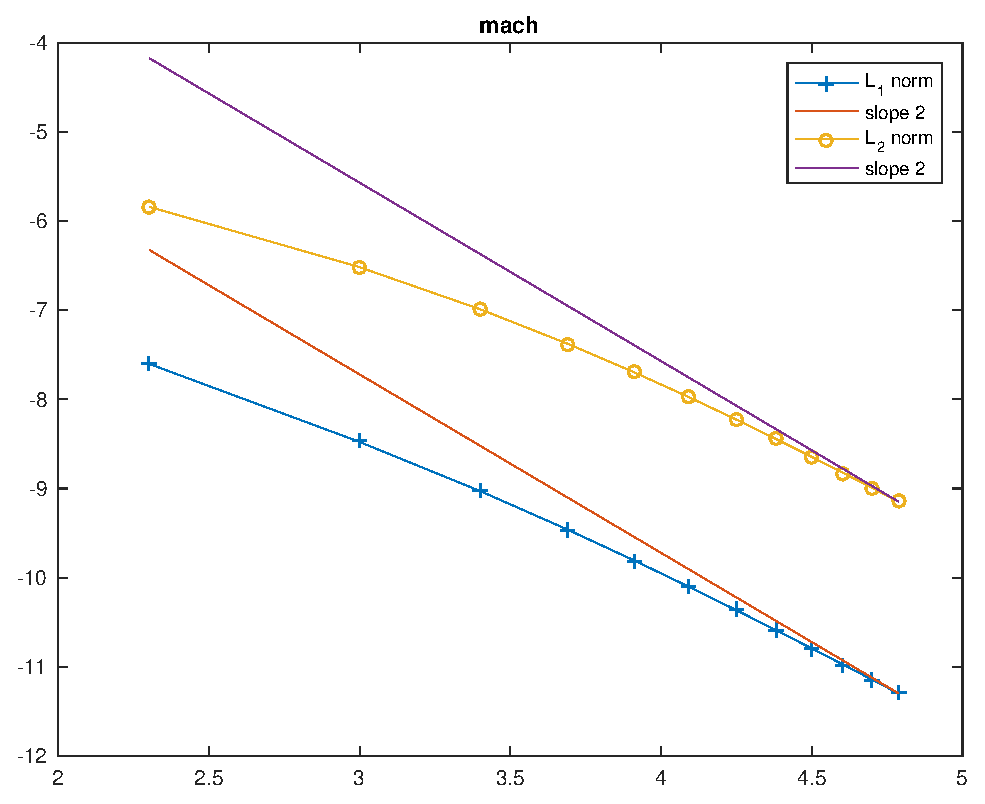
\includegraphics[width=0.4\textwidth]{\FiguresDirnew/mach_pchip.eps}
}
\subfigure[Mat. Temp.]{
      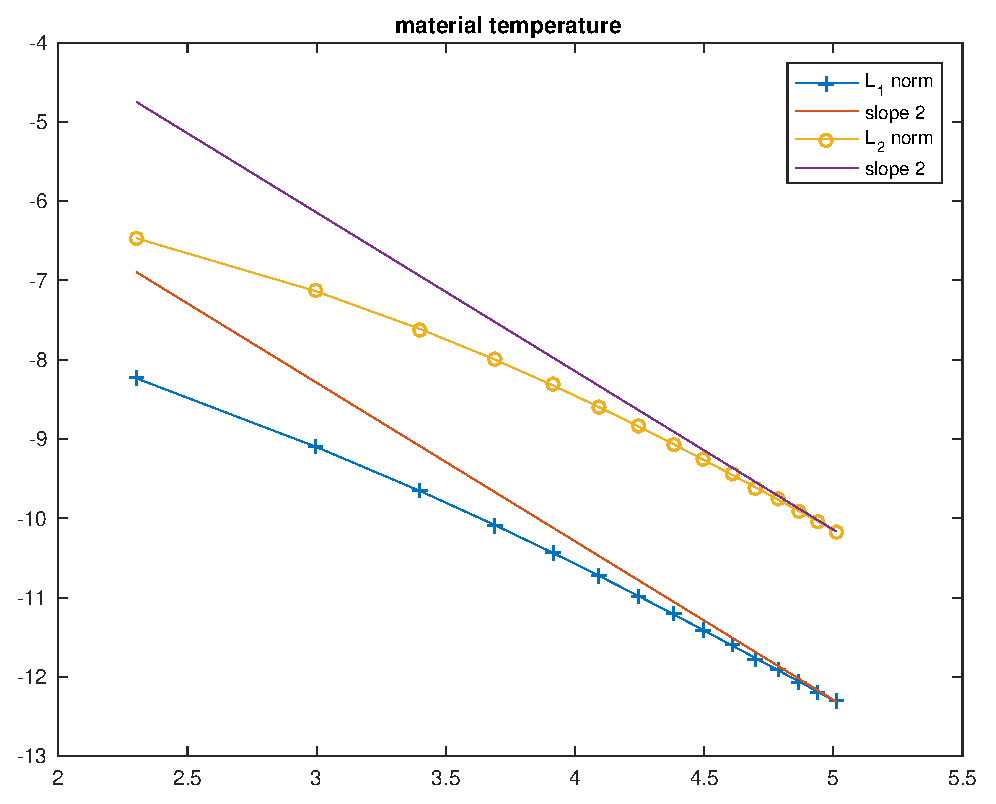
\includegraphics[width=0.4\textwidth]{\FiguresDirnew/material_temperature_pchip.eps}
}
\hspace{1cm}
\subfigure[Radiation Temp.]{
      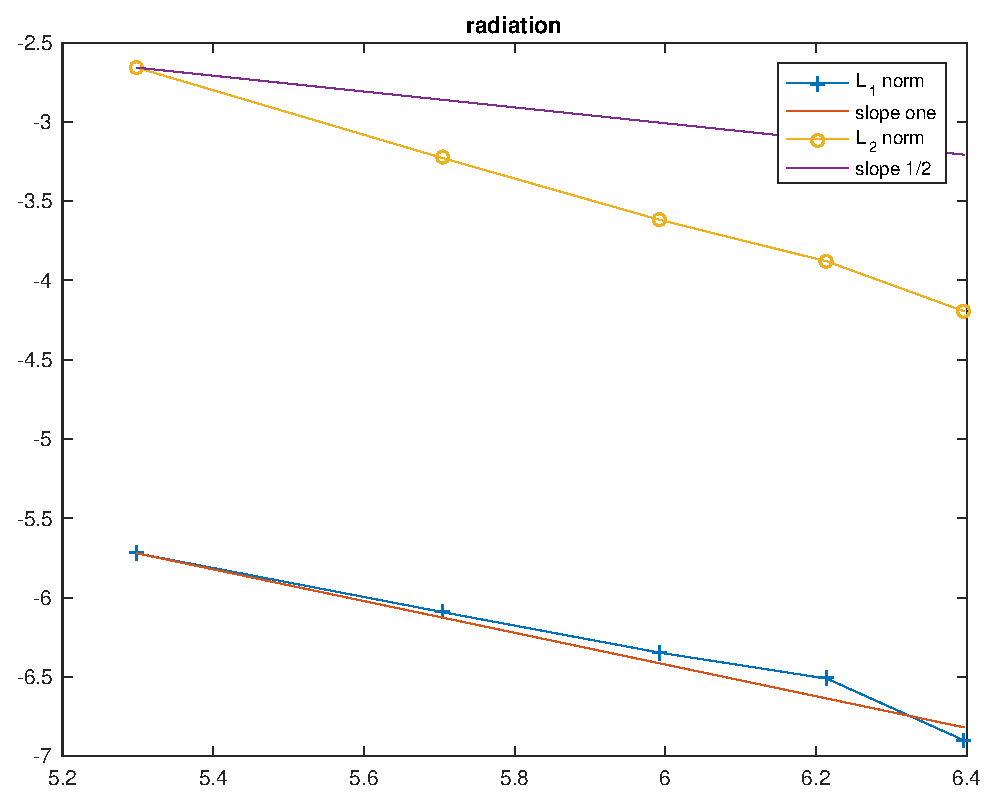
\includegraphics[width=0.4\textwidth]{\FiguresDirnew/radiation_pchip.eps}
}
\end{figure}

\end{frame}
%%%%%%%%%%%%%%%%%%%%%%%%%%%%%%%%%%%%%%%%%%%%%%%%%%%%%%%%%%%%%%%%%%%%%%%%%%%%%%%%%



%%%%%%%%%%%%%%%%%%%%%%%%%%%%%%%%%%%%%%%%%%%%%%%%%%%%%%%%%%%%%%%%%%%%%%%%%%%%%%%%%
\begin{frame}
\frametitle{Mach 3}

% path to figures directory
\newcommand{\FiguresDirnew}{./April4/Mach-3}
\setcounter{subfigure}{0}% Reset subfigure counter
\small{New results, April 4. Now, opacities depend on Temp ??? CFL=0.02}

\begin{figure}[h]
   \centering
\subfigure[Density]{
      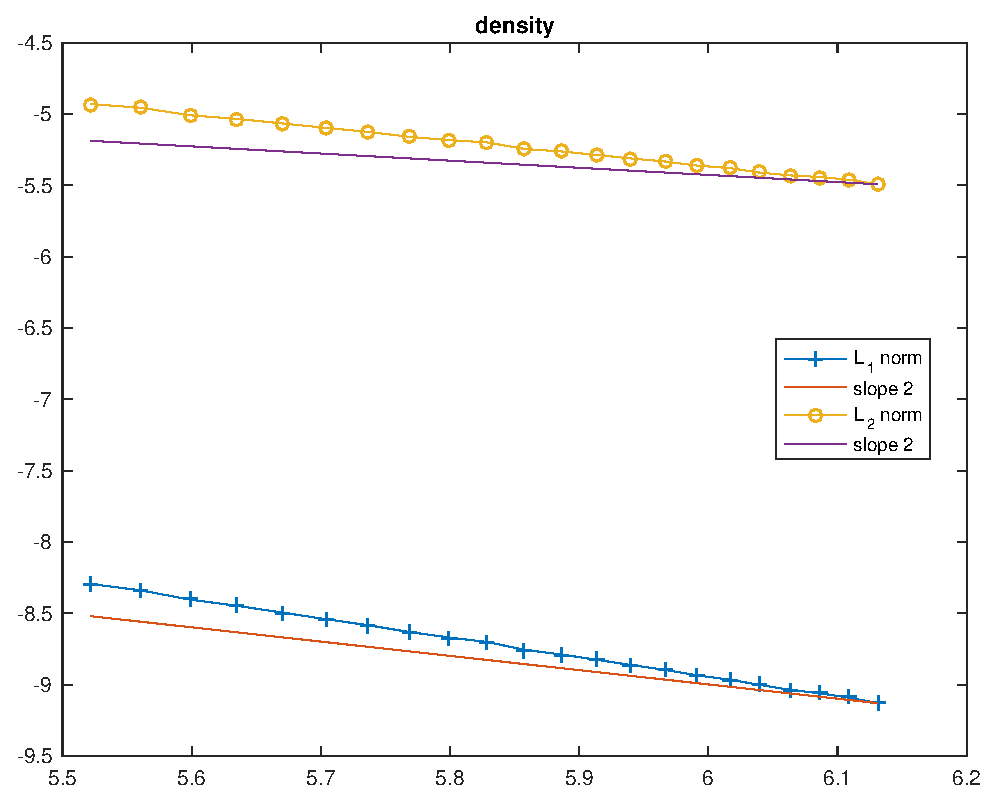
\includegraphics[width=0.4\textwidth]{\FiguresDirnew/density_pchip.eps}
}
\hspace{1cm}
\subfigure[Mach]{
      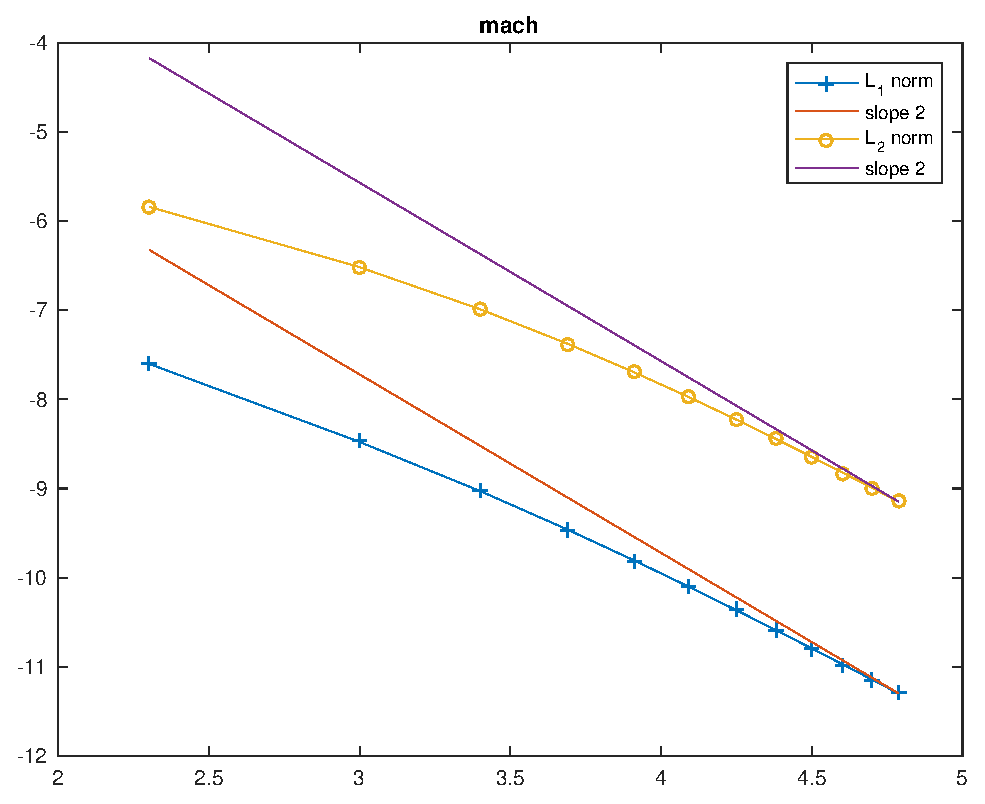
\includegraphics[width=0.4\textwidth]{\FiguresDirnew/mach_pchip.eps}
}
\subfigure[Mat. Temp.]{
      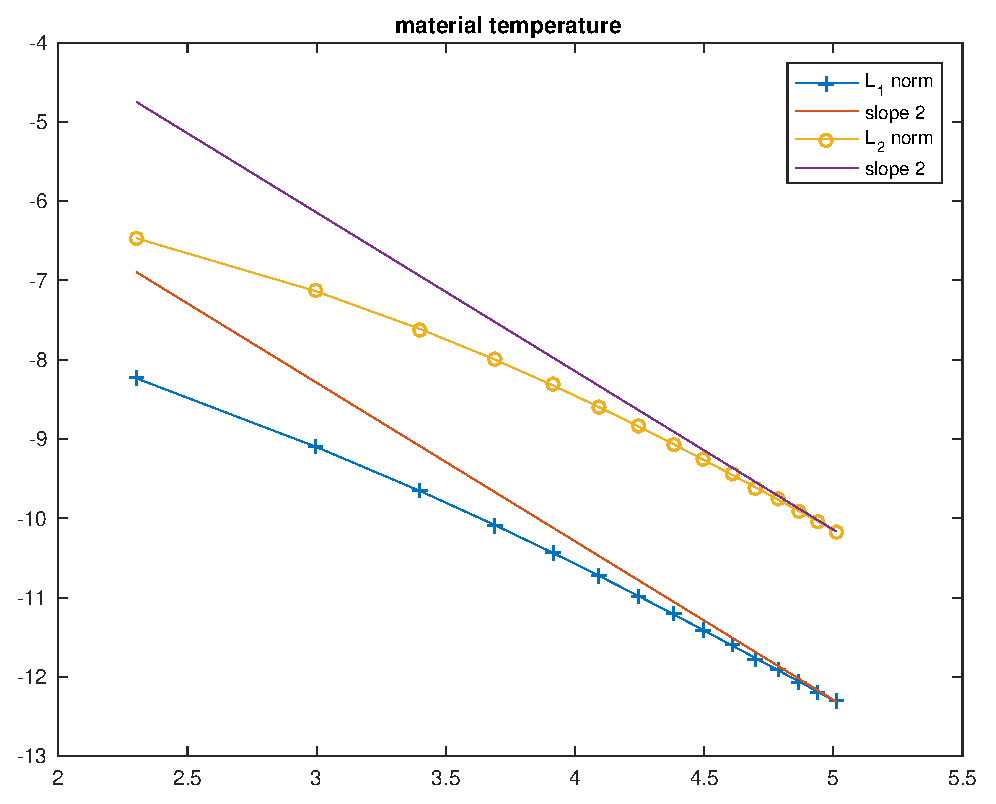
\includegraphics[width=0.4\textwidth]{\FiguresDirnew/material_temperature_pchip.eps}
}
\hspace{1cm}
\subfigure[Radiation Temp.]{
      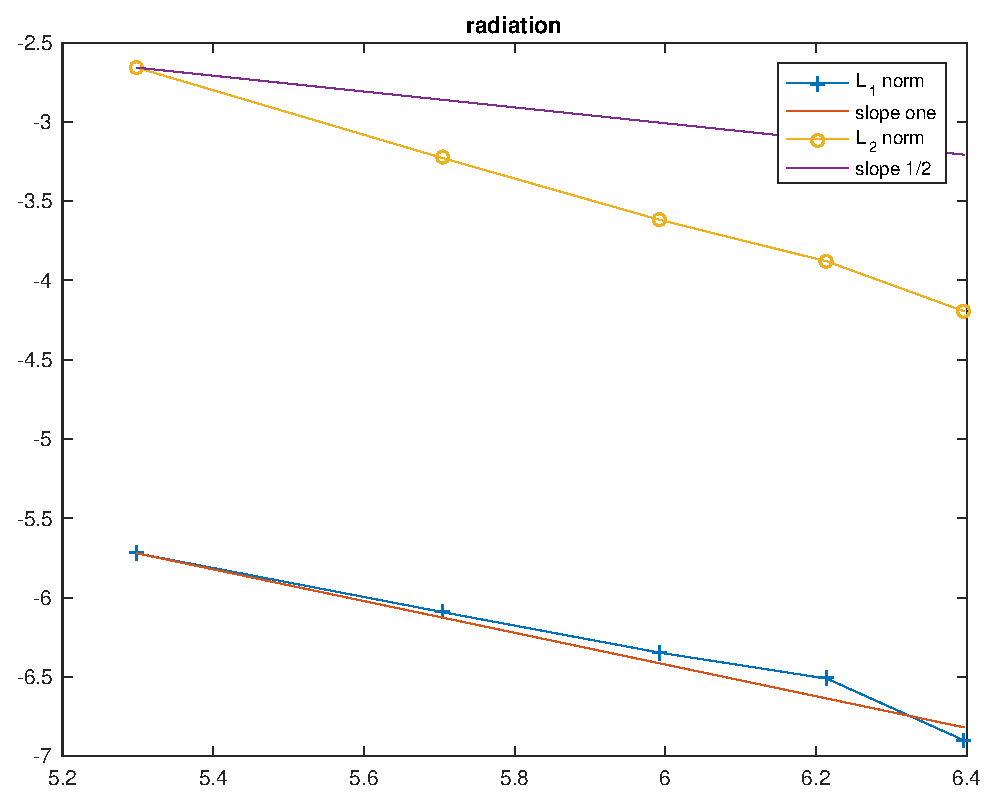
\includegraphics[width=0.4\textwidth]{\FiguresDirnew/radiation_pchip.eps}
}
\end{figure}

\end{frame}
%%%%%%%%%%%%%%%%%%%%%%%%%%%%%%%%%%%%%%%%%%%%%%%%%%%%%%%%%%%%%%%%%%%%%%%%%%%%%%%%%

%%%%%%%%%%%%%%%%%%%%%%%%%%%%%%%%%%%%%%%%%%%%%%%%%%%%%%%%%%%%%%%%%%%%
%%%%%%%%%%%%%%%%%%%%%%%%%%%%%%%%%%%%%%%%%%%%%%%%%%%%%%%%%%%%%%%%%%%%
%%%%%%%%%%%%%%%%%%%%%%%%%%%%%%%%%%%%%%%%%%%%%%%%%%%%%%%%%%%%%%%%%%%%
\end{document}
